\documentclass{article}

%preamble
\usepackage{amsmath}%insert math equation
\usepackage{graphicx} %insert picture
\usepackage{subcaption}%insert pictures at the same place
\usepackage{setspace}%spacing
\usepackage{listings}%code highlighting
\usepackage{color}
\usepackage[T1]{fontenc}
\usepackage{hyperref}%hyperlink
\renewcommand\lstlistingname{Quelltext} % Change language of section name
\lstset{ % General setup for the package
	language=Perl,
	basicstyle=\small\sffamily,
	numbers=left,
 	numberstyle=\tiny,
	frame=tb,
	tabsize=4,
	columns=fixed,
	showstringspaces=false,
	showtabs=false,
	keepspaces,
	commentstyle=\color{red},
	keywordstyle=\color{blue}
}

\title{My first document}
\date{2013-09-01}
\author{John Doe}

%\setcounter{tocdepth}{1} % Show sections
\setcounter{tocdepth}{2} % + subsections
%\setcounter{tocdepth}{3} % + subsubsections
%\setcounter{tocdepth}{4} % + paragraphs
%\setcounter{tocdepth}{5} % + subparagraphs

\begin{document}
	
	\maketitle
	\pagenumbering{gobble}
	\newpage
	\doublespacing
	\tableofcontents
	\singlespacing
	\newpage
	\pagenumbering{arabic}

	\section{Section}

	Hello World!

	\subsection{subsection}
	Structuring a document is easy!

	\section{Section2}

	\subsubsection{subsubsection}

	\paragraph{paragraph}
	\subparagraph{subparagraph}
	\begin{equation}  
		f(x) = x^2
	\end{equation}

	\begin{equation*}  %without numeric mark
		f(x) = x^2
	\end{equation*}
	\section{Section3}

	This formula $f(x) = x^2$ is an example

	\begin{equation*}
		1+2 = 3
	\end{equation*}

	\begin{equation*}
		1 = 3-2
	\end{equation*}

%The align environment will align the equations at the ampersand &. Single equations have to be seperated by a linebreak \\.
	\begin{align*}
		1+2 &= 3\\
		1&= 3-2
	\end{align*}

	\begin{align}
		f(x) &= x^2\\
		g(x) &= \frac{1}{x}\\
		F(x) &= \int^a_b \frac{1}{3}x^3
	\end{align}

	$$\frac{1}{\sqrt{x}}$$
	\begin{equation*}
	%matrices only work within math environments
	\left[
	\begin{matrix}
	1 & 0\\
	0 & 1
	\end{matrix}
	\right]
	[
	\begin{matrix}
	1 & 0\\
	0 & 1
	\end{matrix}
	]
	\end{equation*}

	\begin{figure}[h!]
	  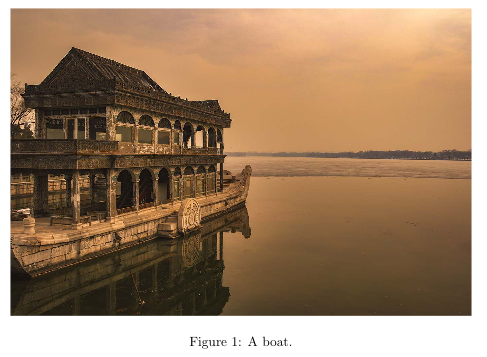
\includegraphics[width=\linewidth]{boat.png}
	  \caption{A boat.}
	  \label{fig:boat1}
	\end{figure}

	Figure \ref{fig:boat1} shows a boat.

	\begin{figure}[h!]
		\centering
		\begin{subfigure}[b]{0.4\linewidth}
			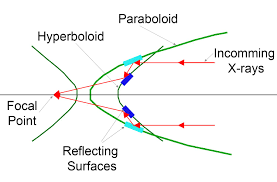
\includegraphics[width=\linewidth]{op1.png}
			\caption{op1.}
		\end{subfigure}
		\begin{subfigure}[b]{0.4\linewidth}
			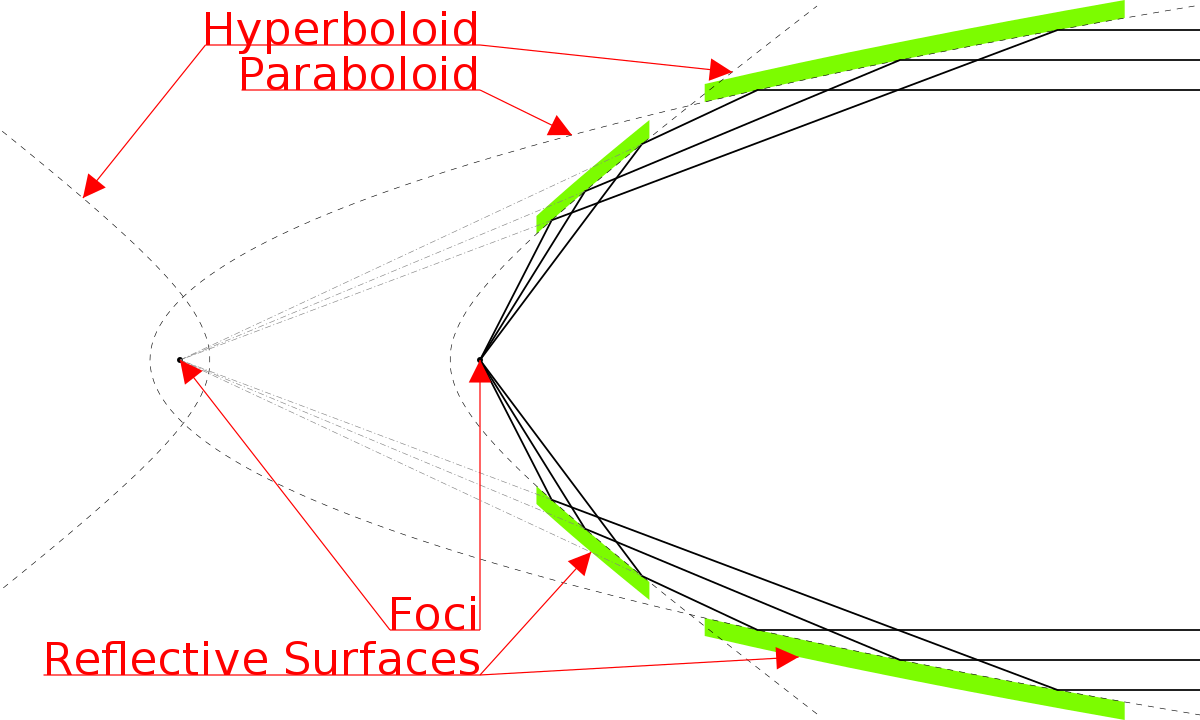
\includegraphics[width=\linewidth]{op2.png}
			\caption{op2.}
		\end{subfigure}
		\caption{Two optical figures}
		\label{fig:ops}
	\end{figure}

	Random citation \cite{Michette2013} embedded in text.

	\newpage

	\bibliography{bibsample}
	\bibliographystyle{ieeetr}

\begin{table}[h!]
  \begin{center}
    \caption{Your first table.}
    \label{tab:table1}
    \begin{tabular}{l|c|r} % <-- Alignments: 1st column left, 2nd middle and 3rd right, with vertical lines in between
      \textbf{Value 1} & \textbf{Value 2} & \textbf{Value 3}\\
      $\alpha$ & $\beta$ & $\gamma$ \\
      \hline
      1 & 1110.1 & a\\
      2 & 10.1 & b\\
      3 & 23.113231 & c\\
    \end{tabular}
  \end{center}
\end{table}

\begin{lstlisting}
#!/usr/bin/perl
print S(@ARGV);sub S{$r=(@_[0]%4==0&&@_[0]%100!=0)||@_[0]%400=0;}
\end{lstlisting}

This is my link: \href{http://www.latex-tutorial.com}{LaTeX-Tutorial}.

\begin{itemize}
	\item One
	\item Two
	\item Three
\end{itemize}

\begin{enumerate}
	\item One
	\item Two
	\item Three
\end{enumerate}

\begin{enumerate}
	\item One
    \begin{enumerate}
    	\item Two
        \item Three
        \item Four
    \end{enumerate}
    \item Five
    \item Six
\end{enumerate}
\end{document}